\documentclass[lettersize,journal]{IEEEtran}
\usepackage[UTF8]{ctex} % 中文支持，需使用 XeLaTeX 编译

\usepackage{amsmath,amsfonts}
\usepackage{algorithmic}
\usepackage{algorithm}
\usepackage{array}
\usepackage[caption=false,font=normalsize,labelfont=sf,textfont=sf]{subfig}
\usepackage{textcomp}
\usepackage{stfloats}
\usepackage{url}
\usepackage{verbatim}
\usepackage{graphicx}
\usepackage{cite}
\graphicspath{{../figures/}}
\hyphenation{op-tical net-works semi-conduc-tor IEEE-Xplore}

\begin{document}

\title{DualCMP：融合与源特定BEV表示下的协同运动预测}

% 手稿（manuscript.md）中未提供作者姓名与所属机构。
\author{}

\maketitle

\begin{abstract}
预测周围智能体的未来运动对自动驾驶的安全性至关重要。车万物（V2X）通信通过共享空间上分离的网联自动驾驶车辆（CAV）的观测信息来增强场景理解。现有协同预测器主要通过两种方式工作：要么融合BEV特征用于感知，要么在预测前关联已跟踪的轨迹。这些流水线分别提升了场景理解与历史运动表示，然而运动预测往往依赖于智能体特定的空间上下文，并且由于感知范围和遮挡的差异，信息量丰富的视角可能因智能体而异。我们提出\textbf{DualCMP}，一个利用融合BEV特征与源特定BEV特征的协同运动预测框架。DualCMP以两种方式使用相同的LiDAR编码：融合BEV特征用于更新持久查询（persistent queries），而每个查询从对齐后的CAV特征图中聚合局部特征。运动锚定解码器将协同上下文与运动历史及智能体间交互相整合，以生成多模态轨迹。在V2V4Real的严格在线评测中，当前seed-20模型取得了5秒minADE$_6$为1.9350 m、minFDE$_6$为3.2465 m的成绩；注意力分析进一步表明，其CAV权重随观测支持与相对几何关系而变化。要将对预测性能的增益归因于源特定表示，仍需进行协议匹配（protocol-matched）的融合BEV对比。
\end{abstract}

\begin{IEEEkeywords}
协同感知，运动预测，车万物通信，持久查询，鸟瞰图表示。
\end{IEEEkeywords}

\section{引言}
\IEEEPARstart{运}{动}预测是自动驾驶的核心组件，因为安全规划依赖于对周围智能体未来运动的预判 \cite{zhou2022hivt,zhou2023qcnet}。预测器利用观测到的智能体状态、邻近智能体以及局部场景上下文来生成多个可能的未来轨迹；而遮挡、稀疏的LiDAR回波以及有限的感知范围都可能使输入不完整 \cite{zhou2022hivt,zhou2023qcnet}。车万物（V2X）通信为接收端提供了来自空间上分离的网联自动驾驶车辆（CAV）的观测 \cite{xu2023v2v4real,wang2020v2vnet}。经过空间对齐后，CAV的观测可以扩展接收端的视距，并为场景理解与预测提供互补的上下文 \cite{wang2020v2vnet,zhou2025v2xpnp}。当预测开始时，表示的选择决定了针对特定目标智能体，哪些协同证据仍然可用。

现有协同运动预测方法在不同的阶段使用CAV观测，并为下游模块提供不同的表示。中间融合方法在对检测与跟踪之前对CAV的BEV特征进行编码与对齐，因此下游模块接收融合后的BEV用于接收端的场景理解 \cite{wang2020v2vnet,wang2025cmp,zhou2025v2xpnp}。通过在统一坐标系中组合多个视角的观测，融合BEV表示支持当前状态估计。第二类工作从各感知流产生的检测结果、跟踪结果或历史轨迹出发，在预测之前进行跨视角关联或轨迹融合；而预测级方法则组合由独立预测器产生的预测假设 \cite{yu2023v2xseq,ruan2024v2xgraph,wu2025copad,zhang2025comtp,wang2025cmp,madjid2026latefusion}。较晚的融合阶段保留了各视角特定的运动历史或预测假设，但在最终协同表示形成之前，密集的空间观测就已经被转换为边界框、轨迹或轨迹特征。图~\ref{fig:introduction}总结了主要区别：中间融合在智能体状态估计之前形成融合BEV，而轨迹融合在感知与跟踪之后，从各视角特定的历史出发。

\begin{figure}[!t]
\centering
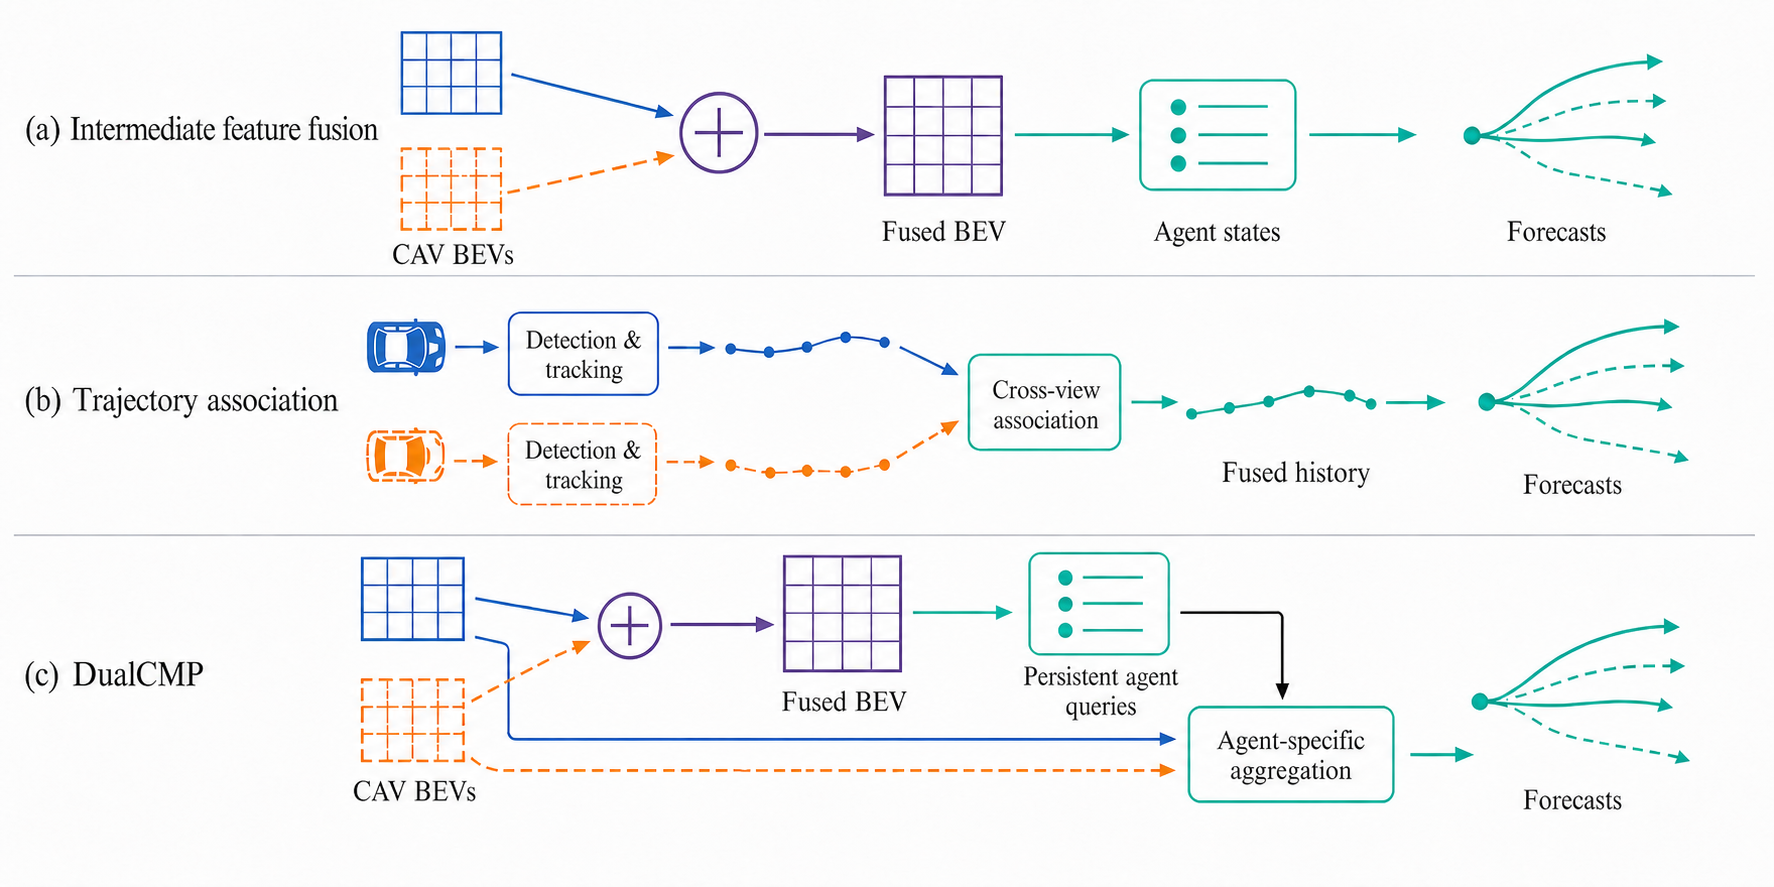
\includegraphics[width=\columnwidth]{dualcmp_introduction_fig1_v3}
\caption{面向运动预测的协同信息融合。(a) 中间融合在智能体状态估计与预测之前聚合对齐后的CAV BEV特征。(b) 轨迹融合在预测之前关联并融合由独立检测与跟踪流水线产生的历史。(c) DualCMP使用融合BEV特征更新持久智能体查询，并对齐CAV特征图以进行以智能体为中心的运动预测。}
\label{fig:introduction}
\end{figure}

在运动预测中，预测器围绕特定目标智能体组织运动历史、邻近智能体与局部上下文 \cite{zhou2022hivt,zhou2023qcnet}。由于每个智能体与观测CAV的空间关系不同，不同视角的重要性可能随目标智能体而变化。对某一智能体提供有用信息的视角，对同一场景中的另一智能体可能信息量较少 \cite{wang2025cmp,ruan2024v2xgraph}。中间融合在融合BEV中保留了空间上下文，但在形成统一的智能体状态时，来源维度不再显式存在。轨迹级和预测级融合保留了各视角特定的历史或局部生成的预测假设，但其协同表示在目标参考建立之后并未暴露出密集的、已对齐到接收端的CAV特征图。因此，这些接口不允许下游预测器针对特定目标检索源特定的空间特征，尽管公共场景表示对于当前状态估计仍然有用。

为了解决这一局限，DualCMP从共享的LiDAR编码器中同时保留两种表示。FuseBEVT将对齐的CAV BEV特征聚合为融合BEV，用于为每个交通智能体更新一个持久查询。查询形成后，运动预测器将查询及其当前边界框作为目标参考，从对齐的CAV特征图中检索局部特征，并与CAV--智能体相对几何相结合。该设计在以接收端为中心地估计当前状态的同时，为预测提供了智能体特定的多视角空间上下文，而无需为各个CAV维护独立的轨迹。运动锚定解码器将协同上下文与有序运动历史及智能体间交互相结合，以生成多模态轨迹。由于持久查询可能包含不同数量的观测历史，且状态估计可能带有噪声，解码器从观测历史导出轨迹锚，并在锚周围预测残差轨迹。我们在严格在线协议下评测完整模型，并使用融合与逐CAV预测输入之间的固定跟踪对比，以检验源特定空间特征的贡献。

主要贡献总结如下：
\begin{enumerate}
\item 我们提出了一个接收端协同运动预测框架，在线处理多CAV LiDAR观测，利用融合BEV测量更新持久智能体查询，并从在线状态而非预计算的跟踪轨迹出发进行预测。
\item 我们开发了智能体特定的CAV特征聚合方法，以目标查询和CAV--智能体相对几何为条件检索局部对齐的BEV特征，同时共享一个LiDAR编码器并为每个智能体保持单一的接收端状态。
\item 我们提出了运动锚定的预测流水线和固定跟踪评测，在融合与逐CAV预测输入下，对匹配的智能体集合联合报告跟踪性能、预测覆盖率和轨迹精度。
\end{enumerate}

本文其余部分组织如下：第二节回顾相关工作，第三节定义协同运动预测问题，第四节介绍DualCMP，第五节报告实验结果。

\section{相关工作}
\subsection{协同感知与预测}

协同感知方法通过交换原始观测、目标输出或中间特征来提升接收端的场景理解。中间融合在空间上下文与通信开销之间取得平衡，是CMP所采用的感知骨干 \cite{wang2025cmp}。CMP通过模块化的检测--跟踪--预测流水线以及预测轨迹的二次交换，将协同感知扩展到运动预测。V2XPnP研究了面向端到端多智能体感知与预测的单步时空融合 \cite{zhou2025v2xpnp}，而UniMM-V2X使用任务特定表示实现感知级与预测级的协同 \cite{souig2026unimm}。

轨迹级方法则从上游感知与跟踪产生的历史轨迹出发。PP-VIC在应用轨迹预测器之前，使用CBMOT融合车辆侧与基础设施侧的轨迹 \cite{yu2023v2xseq}。V2X-Graph学习跨视角关联并融合运动与交互特征 \cite{ruan2024v2xgraph}；CoPAD结合匈牙利匹配与卡尔曼滤波进行多源轨迹融合 \cite{wu2025copad}；Co-MTP在历史域与未来域上进行轨迹融合 \cite{zhang2025comtp}。ViTraj进一步学习车辆侧与基础设施侧的轨迹表示 \cite{you2025vitraj}。预测聚合是CMP和近期晚融合工作 \cite{wang2025cmp,madjid2026latefusion} 中更晚的一种协同形式。DualCMP保留中间融合用于持久状态估计，并复用对齐后的CAV特征图用于以智能体为中心的运动预测。

\subsection{以智能体为中心的运动预测}

运动预测器通常结合时间上的智能体状态、局部场景上下文与社会交互。HiVT将局部上下文提取与全局智能体交互分离，并使用相对几何表示 \cite{zhou2022hivt}。QCNet使用以查询为中心的编码以及提议--精化解码器，其中提议的轨迹为上下文检索提供自适应锚 \cite{zhou2023qcnet}。DualCMP并不直接采用这两个模型：在当前设置下，V2V4Real不提供高精地图（HD map），且DualCMP的输入是在线的持久查询状态，而非真值轨迹历史。我们转而借鉴其架构原则，以组织观测到的运动历史、CAV相对几何、智能体交互以及多模态解码。

\subsection{联合跟踪与预测}

持久目标查询已被用于在单车系统中连接检测、跟踪与预测。预测的运动还可以用于遮挡处理或后续感知，例如PF-Track和ForeSight等方法 \cite{pang2023pftrack,papais2025foresight}。DualCMP则使用持久查询来维护智能体身份，并将预测视为在线跟踪状态的只读消费者。

\section{问题定义}

考虑一个场景，在时刻 \(t\) 有 \(N_t\) 个可用CAV，令 \(r\in\{1,\ldots,N_t\}\) 表示接收端。我们用 \(\mathbf{L}_t^j\) 和 \(\boldsymbol{\xi}_t^j\) 分别表示CAV \(j\) 的LiDAR点云和位姿。从CAV \(j\) 到接收端 \(r\) 的相对变换以及运行时输入为
\[
\mathbf{T}_{j\rightarrow r}^t
=\left(\boldsymbol{\xi}_t^r\right)^{-1}\boldsymbol{\xi}_t^j,
\qquad
\mathcal{X}_r^t=
\left(
\left\{\mathbf{L}_t^j,\mathbf{T}_{j\rightarrow r}^t\right\}_{j=1}^{N_t},
\boldsymbol{\xi}_t^r,\tau_t^r
\right),
\tag{1}
\]
其中 \(\tau_t^r\) 是接收端时间戳。给定 \(\mathcal{X}_r^t\) 和上一时刻的状态，任务是估计周围智能体的当前状态，并在接收端坐标系中预测其未来轨迹。真值边界框、身份标识和未来轨迹仅用于训练与评测，不包含在 \(\mathcal{X}_r^t\) 中。

\section{方法}
\subsection{框架概览}

DualCMP是一个在线协同运动预测框架，按时间顺序处理每个接收端序列。它包含四个主要组件：协同BEV特征编码、持久查询跟踪、智能体特定CAV特征融合以及多模态运动预测。共享的LiDAR编码器为每个可用CAV生成一张BEV特征图。FuseBEVT将这些特征图组合为融合BEV特征，用于当前目标检测与跟踪，而各个CAV的特征仍然可供运动预测分支使用。两个分支因此共享相同的LiDAR特征，但保留不同的表示以服务于各自的任务。

融合BEV特征为每个被跟踪的智能体更新一个持久状态。在获得当前智能体状态之后，每个激活的查询从各个CAV特征图中提取局部特征。运动预测器将聚合后的CAV特征与观测到的状态历史以及其他激活智能体的特征相结合，然后预测多条未来轨迹及其概率。各个CAV的特征在构造运动模态之前，对每个智能体只融合一次；解码器不引入第二次源选择或轨迹精化阶段。运动预测读取当前跟踪状态，但不修改查询分配、状态传播或轨迹管理。

\subsection{协同BEV特征编码}

遵循CMP \cite{wang2025cmp}，我们在体素化之前将每个CAV的点云变换到当前接收端坐标系。共享的PointPillar编码器 \(E_\theta\) 将CAV \(j\) 变换后的点云映射为BEV特征 \(\mathbf{F}_j^t\in\mathbb{R}^{C\times H\times W}\)。CAV特征根据每个样本中有效CAV的数量重新分组，并由FuseBEVT组合：
\[
\mathbf{F}_j^t=E_\theta
\left(\mathbf{T}_{j\rightarrow r}^t\mathbf{L}_t^j\right),
\qquad
\mathbf{F}_{\mathrm{fuse}}^t=
\operatorname{FuseBEVT}
\left(\{\mathbf{F}_j^t\}_{j=1}^{N_t},\mathbf{m}^t\right),
\tag{2}
\]
其中 \(\mathbf{m}^t\) 指示在样本被填充为相同形状时哪些CAV特征是有效的。由于所有点云已经变换到接收端坐标系，\(\mathbf{F}_j^t\) 和 \(\mathbf{F}_{\mathrm{fuse}}^t\) 使用相同的BEV网格。特征编码之后不再施加额外的空间变换。

DualCMP保留(2)式中的两种输出。\(\mathbf{F}_{\mathrm{fuse}}^t\) 上的分类与边界框回归头产生稠密的测量候选（measurement proposals），持久查询解码器使用相同的融合特征估计当前智能体状态。各个特征图 \(\{\mathbf{F}_j^t\}\) 保留了CAV维度，并在跟踪之后提供给运动预测分支。两个分支使用同一个PointPillar编码器；DualCMP既不引入第二个感知骨干，也不为每个CAV维护独立的轨迹。

\subsection{持久查询跟踪}

在时刻 \(t\)，接收端维护一个固定容量的查询库
\[
\mathcal{S}_r^t=
\left\{
\mathbf{q}_i^t,\mathbf{b}_i^t,\mathbf{v}_i^t,
e_i^t,a_i^t,d_i^t,\mathcal{H}_i^t
\right\}_{i=1}^{Q},
\tag{3}
\]
其中 \(\mathbf{q}_i^t\) 是查询特征，\(\mathbf{b}_i^t\in\mathbb{R}^{7}\) 是3D边界框，\(\mathbf{v}_i^t\in\mathbb{R}^{2}\) 是平面速度，\(e_i^t\) 是存在性logit。\(a_i^t\) 和 \(d_i^t\) 分别表示查询年龄和连续缺失测量的次数，\(\mathcal{H}_i^t\) 存储可用的查询与边界框历史。递归状态还记录接收端位姿和时间戳，以便状态可以在相邻接收端帧之间进行变换。每个激活的查询表示一个物理智能体，而非一个CAV观测。

在处理新帧之前，将上一时刻的边界框变换到当前接收端坐标系，并用匀速模型进行传播。\(\mathbf{F}_{\mathrm{fuse}}^t\) 上的稠密头产生当前的测量候选。我们在激活查询与有效候选之间应用距离门控的一对一分配。每个激活查询还有一个私有的空分配（null assignment），防止无效匹配占用对其他查询合适的候选。匹配到的候选为已有查询提供参考边界框，而未匹配的候选则初始化一个非激活的查询槽位。

遵循在线跟踪中使用的持久查询形式 \cite{gu2023vip3d}，可变形注意力解码器从融合BEV特征更新查询特征和状态：
\[
(\widetilde{\mathbf{q}}_i^t,
\widehat{\mathbf{b}}_i^t,
\widehat{\mathbf{v}}_i^t,
\widehat e_i^t)
=D_\phi
\left(
\mathbf{F}_{\mathrm{fuse}}^t,
\mathbf{q}_i^{t,-},
\mathbf{b}_i^{t,-}
\right),
\tag{4}
\]
其中上标 \((- )\) 表示传播后的查询和参考边界框。存在性logit与在解码中心周围采样的稠密分类响应相结合。学习的测量增益将传播的边界框与速度同对应的解码估计值进行组合。轨迹管理负责激活新查询、在有限帧数内保留未匹配查询，并释放过期槽位。当未匹配查询保持激活状态时，其传播状态被追加到在线历史中。运行时身份由系统内部生成，不对应标注身份。激活查询在拥有两条有效状态条目后才有资格进行运动预测。预测轨迹不用于分配、传播、测量更新或轨迹管理步骤。

\subsection{智能体特定CAV特征融合}

融合BEV特征为每个智能体提供一个当前状态，但不再暴露哪些CAV贡献了局部观测。因此，对于运动预测，DualCMP在目标智能体建立后回到各个CAV特征图。设 \(\mathbf{p}_n\in[-1,1]^2\) 表示 \(S\times S\) patch中的一个规则偏移，\(r_p\) 为patch半径。对于智能体 \(i\)，在CAV \(j\) 上的采样为
\[
\mathbf{x}_{in}^t=\mathbf{b}_{i,xy}^t+r_p\mathbf{p}_n,
\qquad
\mathbf{f}_{ijn}^t=
\operatorname{Bilinear}\!\left(\mathbf{F}_j^t,\mathbf{x}_{in}^t\right).
\tag{5}
\]
所有CAV特征图都遵循相同的接收端BEV网格，因此对每个CAV使用相同的度量采样位置。实现中的模型使用半径为 \(4\) m的 \(3\times3\) patch。

融合模块还编码目标智能体与观测CAV之间的几何关系。几何向量 \(\mathbf{g}_{ij}^t\in\mathbb{R}^{7}\) 包含归一化相对位置与距离、智能体相对方位角的正弦与余弦、以及相对航向的正弦与余弦。每个采样特征被投影到查询维度，并与几何和patch位置嵌入相结合：
\[
\mathbf{z}_{ijn}^t=
W_f\mathbf{f}_{ijn}^t
+G(\mathbf{g}_{ij}^t)
+P(\mathbf{p}_n),
\tag{6}
\]
其中 \(W_f\)、\(G\) 和 \(P\) 是学习的投影。当前智能体查询用作注意力查询，CAV patch token构成键与值：
\[
\mathbf{c}_i^t=
\operatorname{LN}_{o}\!\left(
\operatorname{MHA}
\left(
\operatorname{LN}_{q}(\mathbf{q}_i^t),
\{\mathbf{z}_{ijn}^t\}_{j,n},
\{\mathbf{z}_{ijn}^t\}_{j,n}
\right)
\right)
\tag{7}
\]
其中不可用的CAV在softmax运算之前被屏蔽，\(\operatorname{LN}_{q}\) 和 \(\operatorname{LN}_{o}\) 分别表示查询与输出层归一化。模型不使用针对固定CAV索引的学习嵌入；相反，每个CAV的特征由其相对几何来标识。因此，对CAV特征、掩码与变换的联合置换不改变 \(\mathbf{c}_i^t\)。融合结果对每个激活智能体分别计算，且仅提供给运动预测分支；跟踪继续使用 \(\mathbf{F}_{\mathrm{fuse}}^t\)。

\subsection{多模态运动预测}

\textbf{历史编码。} 对每个激活查询，DualCMP存储一个有序的状态序列和有效性掩码。每个历史状态由其相对位置、单步运动、加速度、边界框尺寸、航向、观测时间和速度表示。时间Transformer对可用的历史状态进行编码，产生历史特征 \(\mathbf{h}_i^t\)。缺失的历史位置被屏蔽，不贡献注意力。由于历史是在线形成的，编码器只使用截至当前帧已估计的状态。

跟踪噪声可能使由两个选定状态估计出的速度不稳定。因此，我们将速度 \(\overline{\mathbf{v}}_i^t\) 计算为观测历史中有效成对速度的中位数。我们还计算速度离散度 \(\sigma_{v,i}^t\) 以表征运动变化。查询特征、CAV特征、历史特征、运动特征和当前边界框特征组合为
\[
\mathbf{u}_i^t=
\operatorname{LN}(\mathbf{q}_i^t)
+\alpha_c\operatorname{LN}(\mathbf{c}_i^t)
+\alpha_h\mathbf{h}_i^t
+M(\overline{\mathbf{v}}_i^t,\sigma_{v,i}^t,n_i^t)
+B(\mathbf{b}_i^t),
\tag{8}
\]
其中 \(n_i^t\) 是有效历史状态的数量，\(\alpha_c\) 和 \(\alpha_h\) 是有界的、学习的缩放系数。然后我们对所有有资格进行运动预测的智能体特征应用Transformer编码器。这一步允许每个智能体利用邻近智能体的当前运动特征。

\textbf{运动解码器。} 我们使用速度缩放的运动锚来初始化未来轨迹。对于模态 \(k\) 和未来步 \(h\)，锚为
\[
\mathbf{A}_{ikh}=\gamma_k\overline{\mathbf{v}}_i^t h\Delta t,
\tag{9}
\]
其中 \(\gamma_k\) 是模态 \(k\) 的速度缩放系数。实现中的模型使用 \(\gamma_k\in\{0,0.5,0.75,1,1.25,1.5\}\)。给定学习的模态嵌入 \(\mathbf{m}_k\)，我们构造以智能体为条件的模态特征，而非使用纯加性的模态token。预测头输出每个锚周围的有界位置残差、模态分数、两个标准差以及二元高斯分布的相关系数。设 \(\mathcal{V}_i\) 为有效未来步的集合。模态特征、预测均值和多模态分布为
\[
\begin{aligned}
\mathbf{z}_{ik}^t
&=\mathbf{u}_i^t\odot\left(1+\tanh(\mathbf{m}_k)\right)+\mathbf{m}_k,\\
\boldsymbol{\mu}_{ikh}
&=\mathbf{A}_{ikh}+r_{\max}\tanh
\left(\frac{R_h(\mathbf{z}_{ik}^t)}{r_{\max}}\right),\\
\ell_{ik}
&=U_\pi(\mathbf{z}_{ik}^t),
\qquad
\boldsymbol{\Sigma}_{ikh}
&=U_{\Sigma,h}(\mathbf{z}_{ik}^t),
\qquad
\boldsymbol{\pi}_i=\operatorname{softmax}(\boldsymbol{\ell}_i),\\
p(\mathbf{Y}_i\mid\mathbf{u}_i^t)
&=\sum_{k=1}^{K}\pi_{ik}
\prod_{h\in\mathcal{V}_i}
\mathcal{N}
\left(\mathbf{y}_{ih};
\boldsymbol{\mu}_{ikh},\boldsymbol{\Sigma}_{ikh}\right).
\end{aligned}
\tag{10}
\]
位置残差头初始化为零，因此初始轨迹均值跟随运动锚。解码器还包含一个跨模态层，用于在运动模态之间交换信息。运动提议（motion proposal）与跨模态输出在训练期间均受监督，推理时使用运动提议。

\subsection{训练损失}

我们按接收端序列的时间顺序分两个阶段训练DualCMP。第一阶段使用以下损失训练共享的PointPillar编码器、FuseBEVT、稠密检测头与持久查询跟踪器：
\[
\mathcal{L}_{\mathrm{state}}=
\lambda_{\mathrm{det}}(\mathcal{L}_{\mathrm{cls}}+2\mathcal{L}_{\mathrm{reg}})
+\lambda_{\mathrm{exist}}\mathcal{L}_{\mathrm{exist}}
+\lambda_{\mathrm{box}}\mathcal{L}_{\mathrm{box}}
+\lambda_{\mathrm{vel}}\mathcal{L}_{\mathrm{vel}}
+\lambda_{\mathrm{aux}}\mathcal{L}_{\mathrm{aux}}.
\tag{11}
\]
顺序匹配仅用于构造训练损失。在较早帧中已匹配到的查询在其保持激活期间保持相同的标注分配。匈牙利匹配应用于未匹配的目标和可用的查询槽位。真值身份不传入模型状态。

第二阶段，冻结PointPillar编码器、FuseBEVT、稠密测量路径与持久查询跟踪器。我们训练智能体特定的CAV特征聚合、历史编码器、智能体交互与运动解码器。对于每个预测层 \(l\)，正模态 \(k_i^{*(l)}\) 由预测终点与最终有效目标位置之间的距离来选择。运动预测损失为
\[
\mathcal{L}_{\mathrm{motion}}=
\sum_{l=1}^{L}w_l
\left[
\lambda_{\mathrm{gmm}}
\sum_{i}\sum_{h\in\mathcal{V}_i}
-\log\mathcal{N}
\left(
\mathbf{y}_{ih};
\boldsymbol{\mu}_{ik_i^{*(l)}h}^{(l)},
\boldsymbol{\Sigma}_{ik_i^{*(l)}h}^{(l)}
\right)
+\lambda_{\mathrm{mode}}
\sum_i\operatorname{CE}
\left(\boldsymbol{\ell}_i^{(l)},k_i^{*(l)}\right)
\right],
\tag{12}
\]
其中 \(w_l\) 是层 \(l\) 的损失权重。运动提议与跨模态输出取平均，对应 \(w_1=w_2=0.5\)。不使用源选择标签、可用性损失或轨迹精化损失。

在第二阶段冻结当前状态模块，使所有运动预测变体具有相同的智能体查询、边界框和预测覆盖。推理时，DualCMP按时间顺序处理每个接收端序列，在场景边界处重置查询状态，并在不使用真值标注或预计算跟踪轨迹的情况下预测轨迹。

\section{实验}

\subsection{实验设置}

\textbf{数据集。} 我们在V2V4Real数据集 \cite{xu2023v2v4real} 上进行实验。遵循官方划分，训练集和测试集分别包含32个和9个序列。两辆车都被用作接收端，得到3,420个以接收端为中心的训练片段和3,986个测试帧。在每个时间步，模型仅使用当前和上一时间步可用的LiDAR观测、位姿和时间戳。真值边界框、身份标识和未来轨迹不作为模型输入。我们使用以10 Hz采样的1秒观测历史，并预测未来5秒的轨迹。查询在两次有效观测后接受评测。

\textbf{评测指标。} 每种方法预测六条轨迹。我们使用1秒、3秒和5秒的minADE$_6$和minFDE$_6$作为运动预测指标，数值越低越好。我们还使用2米终点阈值报告漏报率。对于跟踪，我们报告MOTA、基于中心的MOTP、精确率和召回率。预测覆盖率（forecast coverage）是匹配到具有有效预测的激活查询的目标智能体帧所占的百分比。ADE、FDE和漏报率在相同的匹配智能体集合上评测。完整的场景--接收端序列被分配到同一个评测进程，指标的和与计数在归一化之前先进行聚合。

\textbf{实现细节。} PointPillar编码器和FuseBEVT从CMP发布的CoBEVT检查点 \cite{wang2025cmp} 初始化。我们首先训练持久查询跟踪器，然后冻结检测与跟踪模块。运动预测模块训练20个轮次，使用AdamW优化器，初始学习率为 \(10^{-4}\)，权重衰减为 \(10^{-4}\)，两个轮次的预热后余弦衰减。模型在两块NVIDIA RTX 3090 GPU上训练，每块GPU两个片段，两次迭代的梯度累积，以及混合精度。有效批大小为8。所有模型使用相同的阶段一检查点、接收端集合、目标掩码、训练调度和随机种子。报告的结果使用seed 20以及最后一个训练轮次的检查点。DualCMP包含195.68M参数，其中4.75M在运动预测阶段被训练。融合BEV模型具有相同数量的参数。两个模型都使用FuseBEVT接收的压缩BEV特征，因此具有相同的通信输入。

\subsection{主要结果}

我们使用相同的在线跟踪结果，将DualCMP与两个运动预测基线进行比较。Online CV使用当前跟踪速度来预测未来位置。Multiscale Anchors使用第四节E小节描述的六个速度缩放系数，不使用轨迹残差。DualCMP使用相同的锚以及第四节描述的运动预测模块。

\begin{table*}[t]
\centering
\caption{V2V4Real测试集上严格在线设置下的运动预测结果。ADE和FDE以米为单位。所有方法使用相同的在线跟踪结果和评测智能体集合。}
\label{tab:main_results}
\resizebox{\textwidth}{!}{%
\begin{tabular}{llcccccc}
\hline
方法 & 预测信息 & \multicolumn{3}{c}{minADE$_6$ $\downarrow$} & \multicolumn{3}{c}{minFDE$_6$ $\downarrow$} \\
\cline{3-8}
 & & 1 s & 3 s & 5 s & 1 s & 3 s & 5 s \\
\hline
Online CV & 查询历史 & 1.2719 & 2.5910 & 3.8351 & 1.8525 & 4.8452 & 7.5505 \\
Multiscale Anchors & 查询历史 & 0.8626 & 1.4673 & 2.0384 & 1.0797 & 2.3704 & 3.5604 \\
DualCMP (ours) & 融合与逐CAV BEV & \textbf{0.8515} & \textbf{1.4083} & \textbf{1.9350} & \textbf{1.0310} & \textbf{2.1841} & \textbf{3.2465} \\
\hline
\end{tabular}}
\end{table*}

表~\ref{tab:main_results}展示了运动预测结果。与Online CV相比，Multiscale Anchors在1秒、3秒和5秒时分别将minFDE$_6$降低了41.71\%、51.08\%和52.85\%。与Multiscale Anchors相比，DualCMP进一步将minFDE$_6$降低了4.51\%、7.86\%和8.82\%。在5秒时，DualCMP取得了1.9350 m的minADE$_6$和3.2465 m的minFDE$_6$。1秒、3秒和5秒的漏报率分别为10.78\%、27.50\%和34.18\%。共享跟踪器取得了65.04\%的MOTA、0.7263 m的MOTP、84.86\%的精确率、81.08\%的召回率以及80.49\%的预测覆盖率。这些结果表明，在相同的在线跟踪设置下，完整的运动预测模型改进了锚轨迹。

\subsection{消融实验}

我们进行消融实验以评估预测表示与特征聚合。融合BEV模型从 \(\mathbf{F}_{\mathrm{fuse}}^t\) 中采样以智能体为中心的patch。逐CAV均值模型对从对齐CAV特征图中采样的以智能体为中心的特征求平均。DualCMP使用智能体查询和智能体--CAV相对几何来聚合逐CAV的patch特征。所有模型使用相同的冻结跟踪器、运动历史、运动锚、预测头、训练调度和评测智能体集合。融合BEV模型和DualCMP模型还使用相同的特征投影与预测参数。

\begin{table*}[t]
\centering
\caption{预测表示与特征聚合的消融实验。最后三列分别报告仅接收端可见、仅伙伴端可见和共享智能体的5秒minFDE$_6$。所有模型使用相同的跟踪器和评测智能体集合。}
\label{tab:representation_ablation}
\resizebox{\textwidth}{!}{%
\begin{tabular}{llccccc}
\hline
预测表示 & 聚合 & minADE$_6$@5s $\downarrow$ & minFDE$_6$@5s $\downarrow$ & 仅接收端 & 仅伙伴端 & 共享 \\
\hline
融合BEV & 智能体patch & -- & -- & -- & -- & -- \\
逐CAV BEV & 均值 & -- & -- & -- & -- & -- \\
逐CAV BEV & 查询与几何 & 1.9350 & 3.2465 & 2.7109 & 5.0998 & 2.7003 \\
\hline
\end{tabular}}
\end{table*}

由于融合BEV模型和逐CAV均值模型的20轮评测尚未完成，其结果不予报告。因此，当前结果未能表明逐CAV BEV特征相比融合BEV特征或均值聚合是否改进了运动预测。

我们进一步评估DualCMP的注意力权重。仅接收端可见、仅伙伴端可见和共享智能体根据两个CAV的LiDAR点云支持来定义。伙伴注意力质量为分配给伙伴CAV的九个patch权重之和。图~\ref{fig:cooperative_analysis}(a)显示，仅接收端可见、仅伙伴端可见和共享智能体的伙伴注意力质量中位数分别为0.3706、0.5988和0.4839。图~\ref{fig:cooperative_analysis}(b)按接收端--智能体距离与伙伴--智能体距离之差对智能体进行分组。当智能体离伙伴CAV更近时，平均伙伴注意力质量从0.3600增加到0.5642。这些结果表明，注意力权重随观测支持和智能体--CAV相对距离而变化。注意力权重并未提供表~\ref{tab:representation_ablation}中三个模型之间预测精度的对比。

\begin{figure*}[t]
\centering
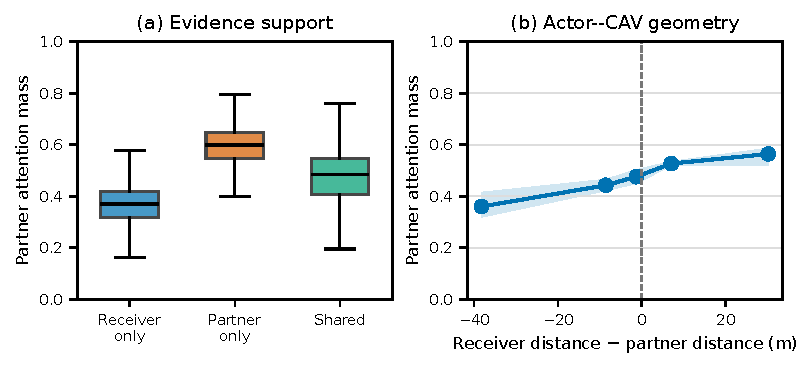
\includegraphics[width=0.78\textwidth]{dualcmp_attention_analysis}
\caption{V2V4Real测试集上的注意力权重。(a) 仅接收端可见、仅伙伴端可见和共享智能体的伙伴注意力质量。中线、箱体和须分别表示中位数、四分位距和1.5倍四分位距范围。(b) 五组智能体--CAV相对距离的平均伙伴注意力质量。阴影区域表示95\%置信区间。正的相对距离表示智能体离伙伴CAV更近。}
\label{fig:cooperative_analysis}
\end{figure*}

\subsection{定性结果}

我们在图~\ref{fig:attention_examples}中提供V2V4Real测试集上的定性结果。我们选择一个仅伙伴端可见智能体和一个共享智能体。每个被选智能体至少具有四次观测、完整的5秒未来轨迹，且未来位移至少为5 m。在每组中，我们选择5秒minFDE$_6$最接近组中位数的示例。融合BEV面板显示目标性响应与跟踪状态。CAV面板显示以智能体为中心的特征图与注意力权重。最后一个面板显示观测轨迹、真值轨迹、六条预测轨迹及其概率。

\begin{figure*}[t]
\centering
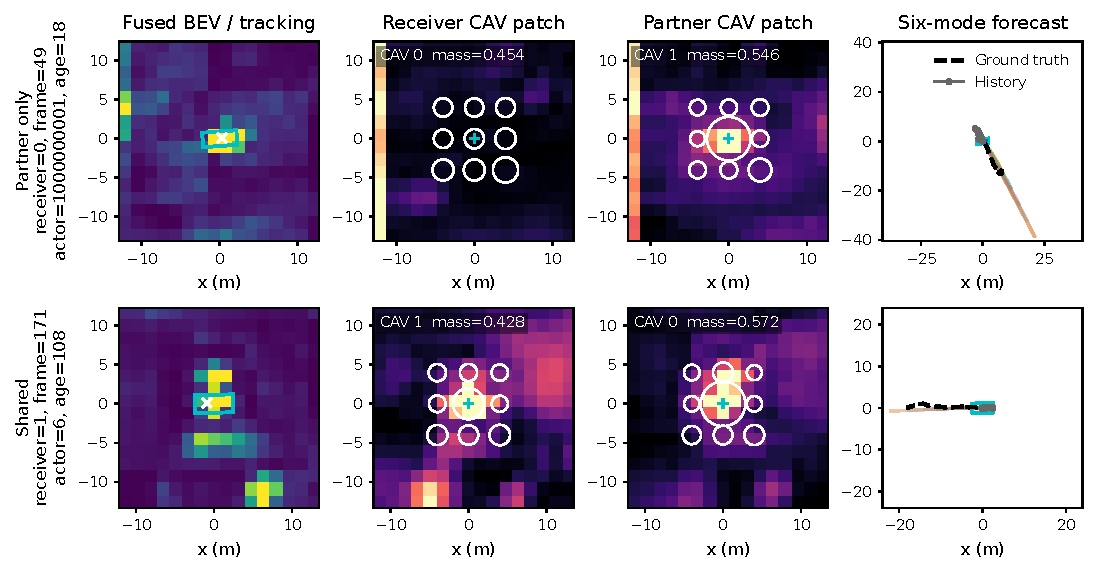
\includegraphics[width=\textwidth]{dualcmp_attention_examples}
\caption{DualCMP在V2V4Real测试集上的定性结果。每行显示一个被跟踪的智能体。第一列显示融合BEV的目标性响应与跟踪状态。第二、三列显示对齐到接收端的CAV特征图。圆的面积表示注意力权重，每个面板报告九个注意力权重之和。最后一列显示灰色观测轨迹、黑色虚线真值轨迹以及六条预测轨迹，每条预测轨迹的不透明度表示其概率。}
\label{fig:attention_examples}
\end{figure*}

\section{结论}

本文提出了DualCMP，一个基于LiDAR的协同跟踪与运动预测框架，将融合与源特定的BEV表示分配给不同任务。FuseBEVT为一个持久查询库提供公共的当前状态测量，而对齐到接收端的逐CAV特征在每个被跟踪智能体周围采样并聚合用于预测。所得的智能体上下文与有序在线历史、智能体交互和运动锚相结合，生成六模态的5秒轨迹，且预测的未来不反馈到跟踪中。在V2V4Real的严格在线协议下，当前seed-20模型在保持65.04\% MOTA和80.49\%预测覆盖率的同时，取得了5秒minADE$_6$为1.9350 m、minFDE$_6$为3.2465 m的成绩。学习得到的源权重随观测支持和CAV--智能体相对距离变化，表明源聚合并未退化为固定平均。要判断所保留的源表示是否提供可复现的预测优势，仍需要协议匹配的融合BEV对比以及更多随机种子。当前研究仅限于单一数据集上的两个同步CAV；异步通信和更大的协同群体留待未来工作。

\begin{thebibliography}{00}
\bibitem{xu2023v2v4real}
R.~Xu \emph{et al.}, ``V2V4Real: A Real-World Large-Scale Dataset for Vehicle-to-Vehicle Cooperative Perception,'' in \emph{Proc. IEEE/CVF Conf. Comput. Vis. Pattern Recognit.}, 2023.

\bibitem{wang2025cmp}
Z.~Wang \emph{et al.}, ``CMP: Cooperative Motion Prediction With Multi-Agent Communication,'' \emph{IEEE Robot. Autom. Lett.}, vol.~10, no.~4, pp.~3876--3883, 2025.

\bibitem{zhou2025v2xpnp}
Z.~Zhou \emph{et al.}, ``V2XPnP: Vehicle-to-Everything Spatio-Temporal Fusion for Multi-Agent Perception and Prediction,'' in \emph{Proc. IEEE/CVF Int. Conf. Comput. Vis.}, 2025.

\bibitem{souig2026unimm}
S.~Souig \emph{et al.}, ``UniMM-V2X: MoE-Enhanced Multi-Level Fusion for End-to-End Cooperative Autonomous Driving,'' in \emph{Proc. AAAI Conf. Artif. Intell.}, 2026.

\bibitem{zhou2023qcnet}
Z.~Zhou, J.~Wang, Y.-H.~Li, and Y.-K.~Huang, ``Query-Centric Trajectory Prediction,'' in \emph{Proc. IEEE/CVF Conf. Comput. Vis. Pattern Recognit.}, 2023.

\bibitem{zhou2022hivt}
Z.~Zhou \emph{et al.}, ``HiVT: Hierarchical Vector Transformer for Multi-Agent Motion Prediction,'' in \emph{Proc. IEEE/CVF Conf. Comput. Vis. Pattern Recognit.}, 2022.

\bibitem{pang2023pftrack}
Z.~Pang \emph{et al.}, ``Standing Between Past and Future: Spatio-Temporal Modeling for Multi-Camera 3D Multi-Object Tracking,'' in \emph{Proc. IEEE/CVF Conf. Comput. Vis. Pattern Recognit.}, 2023.

\bibitem{papais2025foresight}
S.~Papais \emph{et al.}, ``ForeSight: Multi-View Streaming Joint Object Detection and Trajectory Forecasting,'' in \emph{Proc. IEEE/CVF Int. Conf. Comput. Vis.}, 2025.

\bibitem{wang2020v2vnet}
T.-H.~Wang \emph{et al.}, ``V2VNet: Vehicle-to-Vehicle Communication for Joint Perception and Prediction,'' in \emph{Proc. Eur. Conf. Comput. Vis.}, 2020.

\bibitem{gu2023vip3d}
J.~Gu \emph{et al.}, ``ViP3D: End-to-End Visual Trajectory Prediction via 3D Agent Queries,'' in \emph{Proc. IEEE/CVF Conf. Comput. Vis. Pattern Recognit.}, 2023.

\bibitem{ruan2024v2xgraph}
H.~Ruan, H.~Yu, W.~Yang, S.~Fan, and Z.~Nie, ``Learning Cooperative Trajectory Representations for Motion Forecasting,'' in \emph{Adv. Neural Inf. Process. Syst.}, 2024.

\bibitem{you2025vitraj}
S.~You, L.~Weng, and F.~Gao, ``ViTraj: Learning Dual-Side Representations for Vehicle-Infrastructure Cooperative Trajectory Prediction,'' in \emph{Proc. ACM Multimedia}, 2025.

\bibitem{madjid2026latefusion}
N.~A.~Madjid \emph{et al.}, ``Collaborative Trajectory Prediction via Late Fusion,'' arXiv preprint arXiv:2604.22973, 2026.

\bibitem{yu2023v2xseq}
H.~Yu \emph{et al.}, ``V2X-Seq: A Large-Scale Sequential Dataset for Vehicle-Infrastructure Cooperative Perception and Forecasting,'' in \emph{Proc. IEEE/CVF Conf. Comput. Vis. Pattern Recognit.}, 2023.

\bibitem{wu2025copad}
K.~Wu, J.~Qiao, and Y.~Zhang, ``CoPAD: Multi-Source Trajectory Fusion and Cooperative Trajectory Prediction With Anchor-Oriented Decoder in V2X Scenarios,'' in \emph{Proc. IEEE/RSJ Int. Conf. Intell. Robots Syst.}, 2025.

\bibitem{zhang2025comtp}
X.~Zhang \emph{et al.}, ``Co-MTP: A Cooperative Trajectory Prediction Framework With Multi-Temporal Fusion for Autonomous Driving,'' in \emph{Proc. IEEE Int. Conf. Robot. Autom.}, 2025.

\bibitem{shi2022mtr}
S.~Shi \emph{et al.}, ``Motion Transformer With Global Intention Localization and Local Movement Refinement,'' in \emph{Adv. Neural Inf. Process. Syst.}, 2022.
\end{thebibliography}

\end{document}